
\begin{frame}
  \frametitle{Training Set Database: Labels}
    \begin{adjustwidth}{-15pt}{-10pt}
    \begin{block}{ORIGEN designations for reactor technologies and fuel assemblies:}
      \begin{table}
        \scriptsize
        \centering
        \begin{tabular}{@{}lll@{}}
        \toprule
          \textbf{PWR} & \textbf{BWR}  & \textbf{PHWR} \\ \toprule
          CE14x14      & GE7x7-0       & CANDU19       \\
          W17x17       & Abb8x8-1      & CANDU28       \\
          S18x18       & Atrium10x10-9 & CANDU37       \\
          BW15x15      & SVEA64-1      &               \\
          VVER440      &               &               \\
          VVER1000     &               &               \\ \bottomrule
        \end{tabular}
      \end{table}
    \end{block}
    %\vspace{-10pt}
    \begin{block}{Simulation parameters for ORIGEN input files:}
      \begin{table}
        \scriptsize
        \centering
        \begin{tabular}{@{}llll@{}}
          \toprule
          & \textbf{PWR}              & \textbf{BWR}              & \textbf{PHWR}        \\  \toprule
          Power Density [$MW/MTU$]                        
          & \{25, 35, 41\}            & \{10, 22\}                & \{2.2, 18, 22\}      \\
          \boxalert{Burnup} [$GWd/MTU$]                   
          & 2--68, 21 steps           & 1--68, 28 steps           & 0.45--12.6, 28 steps \\
          Moderator Density [$g/cm^3$]                    
          & 0.71                      & \{0.1, 0.3, 0.5, 0.7\}    & 0.84                 \\
          \boxalert{Enrichment} [$\%\:{}^{235}{\text{U}}$]
          & \{0.5, 1.5, 2, 3, 4, 5\}  & \{0.5, 1.5, 2, 3, 4, 5\}  & 0.711                \\
          \boxalert{Cooling Time} [$days$]                
          & \multicolumn{3}{c}{0--6000 in 100-day steps}                                 \\ \bottomrule
        \end{tabular}
      \end{table}
    \end{block}
    \end{adjustwidth}
\end{frame}


\begin{frame}
  \frametitle{Training Set Database: Labels}
  \begin{adjustwidth}{-15pt}{-10pt}
  \begin{minipage}{0.8\textwidth}
    %\vspace{-8pt}
    \begin{figure}
      \centering
        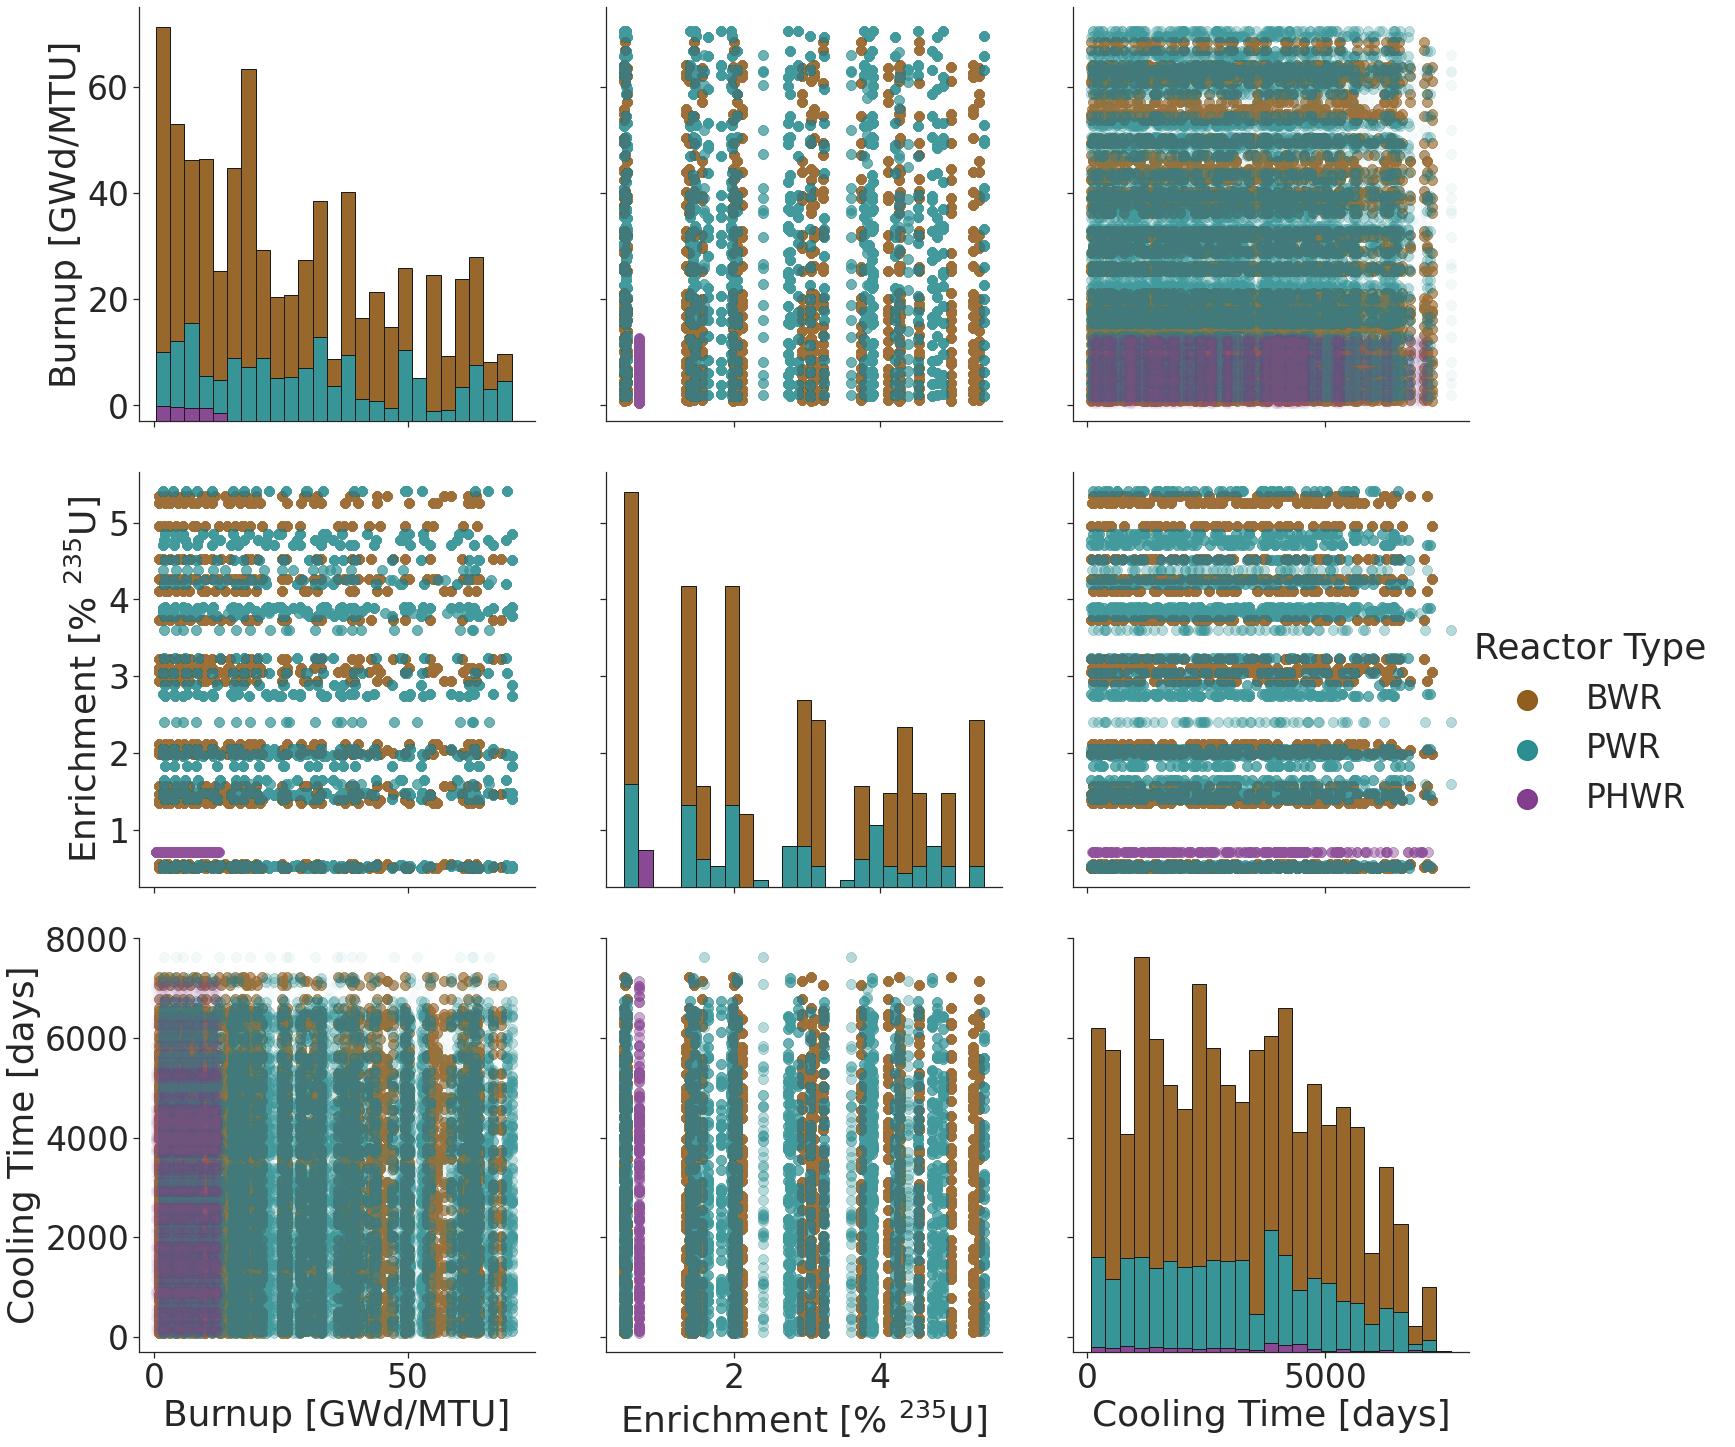
\includegraphics[height=0.85\textheight]{./figures/histogram_scatter_trainset_viz.png}
    \end{figure}
  \end{minipage}%
  \hfill
  \begin{minipage}{0.27\textwidth}
    \small
    Training Set: \\ $4.5 \times 10^5$ entries
    \begin{itemize}
      \small{
      \item PWR: 26.8\% (120960)
      \item BWR: 71.6\% (322560)
      \item PHWR: 1.5\% (6720)
      }
    \end{itemize}
  \end{minipage}
  \end{adjustwidth}
\end{frame}

\begin{frame}
  \frametitle{Training Set Database: Features}
    %\begin{adjustwidth}{-10pt}{0pt}
    \begin{block}{Nuclide masses saved from ORIGEN simulations:}
      \begin{table}
        \small
        \centering
        \renewcommand{\arraystretch}{1.3}
        \begin{tabular}{@{}|l|l|l|l|l|l|l|l|@{}}
          \hline
          \allbold{${}^{241}\text{Am}$} & ${}^{242m}\text{Am}$ &
          \allbold{${}^{243}\text{Am}$} & ${}^{242}\text{Cm}$ &
          \allbold{${}^{244}\text{Cm}$} & \allbold{${}^{134}\text{Cs}$} &
          \allbold{${}^{137}\text{Cs}$} & \allbold{${}^{154}\text{Eu}$} \\  
          \hline
          ${}^{143}\text{Nd}$ & ${}^{144}\text{Nd}$ & ${}^{145}\text{Nd}$ &
          ${}^{146}\text{Nd}$ & ${}^{148}\text{Nd}$ & ${}^{150}\text{Nd}$ &
          \allbold{${}^{237}\text{Np}$} & \allbold{${}^{238}\text{Pu}$} \\ 
          \hline
          \allbold{${}^{239}\text{Pu}$} & \allbold{${}^{240}\text{Pu}$} &
          ${}^{241}\text{Pu}$ & ${}^{242}\text{Pu}$ & ${}^{147}\text{Sm}$ &
          ${}^{149}\text{Sm}$ & ${}^{150}\text{Sm}$ & ${}^{151}\text{Sm}$ \\ 
          \hline
          ${}^{152}\text{Sm}$ & \allbold{${}^{234}\text{U}$} &
          \allbold{${}^{235}\text{U}$} & ${}^{236}\text{U}$ & ${}^{238}\text{U}$ &  &
          & \\  
          \hline
        \end{tabular}
      \end{table}
    \end{block}
    \begin{block}{Nuclide activities saved from ORIGEN simulations:}
      \begin{table}
        \small
        \centering
        \renewcommand{\arraystretch}{1.3}
        \begin{tabular}{@{}|l|l|l|l|l|l|l|l|@{}}
          \hline
          ${}^{227}\text{Ac}$ & \allbold{${}^{241}\text{Am}$} &
          \allbold{${}^{243}\text{Am}$} & ${}^{133}\text{Ba}$ & ${}^{249}\text{Cf}$ &
          ${}^{252}\text{Cf}$ & ${}^{243}\text{Cm}$ & \allbold{${}^{244}\text{Cm}$} \\ 
          \hline
          ${}^{245}\text{Cm}$ & \allbold{${}^{134}\text{Cs}$} &
          \allbold{${}^{137}\text{Cs}$} & ${}^{152}\text{Eu}$ &
          \allbold{${}^{154}\text{Eu}$} & ${}^{166m}\text{Ho}$ & ${}^{85}\text{Kr}$ &
          ${}^{94}\text{Nb}$ \\ 
          \hline
          ${}^{236}\text{Np}$ & \allbold{${}^{237}\text{Np}$} & ${}^{231}\text{Pa}$ &
          ${}^{146}\text{Pm}$ & ${}^{236}\text{Pu}$ & \allbold{${}^{238}\text{Pu}$} &
          \allbold{${}^{239}\text{Pu}$} & \allbold{${}^{240}\text{Pu}$} \\ 
          \hline
          ${}^{226}\text{Ra}$ & ${}^{125}\text{Sb}$ & ${}^{228}\text{Th}$ &
          ${}^{229}\text{Th}$ & ${}^{232}\text{U}$  & ${}^{233}\text{U}$ &
          \allbold{${}^{234}\text{U}$}  & \allbold{${}^{235}\text{U}$}  \\ 
          \hline
        \end{tabular}
      \end{table}
    \end{block}
    %\end{adjustwidth}
\end{frame}

